2015\chapter[Generalidades]{Generalidades sobre la marcha}

El siguiente capítulo pretende introducir al lector los conceptos fundamentales relacionados a la marcha y su estudio. Además de los avances tecnológicos en el área y el estado de estos.

\section{¿Qué es la marcha?}

Por \emph{marcha} se entiende el acto de desplazarse utilizando las extremidades corporales. Según \cite{menz} la marcha consiste de cuatro tareas: (1) inicio y terminación de los movimientos locomotores, (2) generación de movimientos continuos para desplazarse hacia adelante, (3) mantenimiento del equilibrio y (4) adaptabilidad al ambiente. Para \cite{perry} al caminar se utiliza una secuencia de movimientos de las extremidades, con el fin de mover el cuerpo hacia adelante y mantener la estabilidad. Cada uno de estos ciclos (de la secuencia) involucra la interacción de las dos extremidades inferiores, compuestas de varios segmentos, y la masa total del cuerpo. El estudio de la marcha consiste en la identificación de patrones de movimiento generados en la marcha y la segmentación del ciclo.

Es posible utilizar la física clásica para estudiar la marcha. Se puede describir la cinemática de la marcha al determinar las velocidades y aceleraciones de los segmentos rígidos del cuerpo; también se puede describir la dinámica de la marcha al determinar las fuerzas que actúan sobre los segmentos rígidos. Así, la marcha se estudia de dos maneras principales: el vector de fuerza recíproca generado por el suelo al soportar el peso del cuerpo y las velocidades y aceleraciones de las principales uniones involucradas en la marcha. \citep{perry}

Ambas descripciones, cinemática y dinámica, se pueden utilizar para segmentar el ciclo de la marcha. \cite{perry} lo divide según se muestra en la tabla \ref{tab:ciclo_marcha}, además la figura \ref{fig:ciclo_marcha} muestra imágenes tomadas del mismo autor. A pesar del posible significado \emph{psicológico} de las fases detalladas en la tabla \ref{tab:ciclo_marcha} y la figura \ref{fig:ciclo_marcha}, si es posible encontrar un significado físico en el ciclo de la marcha. Considere la figura \ref{fig:menz_acc_ver}, tomada de \citep{menz}.


\begin{table}
    \centering
    \caption{Ciclo de la marcha según \citep{perry}}
    \label{tab:ciclo_marcha}
    \begin{tabular}{l l l}
        \toprule
        Función & Fase & Descripción \\
        \midrule
        Aceptación de la carga & Contacto Inicial & Justo cuando el pie toca el suelo \\
                               & Respuesta a la carga & El otro comienza el balanceo \\
        Soporte & Soporte medio & El centro de masa se alinea con el pié \\
                & Soporte final & El centro de masa sobrepasa el piel \\
        Avance del miembro & pre-balanceo & Se transfiere la carga al otro pie \\
                           & balanceo inicial & Se levanta el pie y avanza \\
                           & balanceo medio   & El pie sobrepasa al otro \\
                           & balanceo final   & Posición apta para contacto inicial \\
        \bottomrule
    \end{tabular}
\end{table}

\begin{figure}
    \centering
    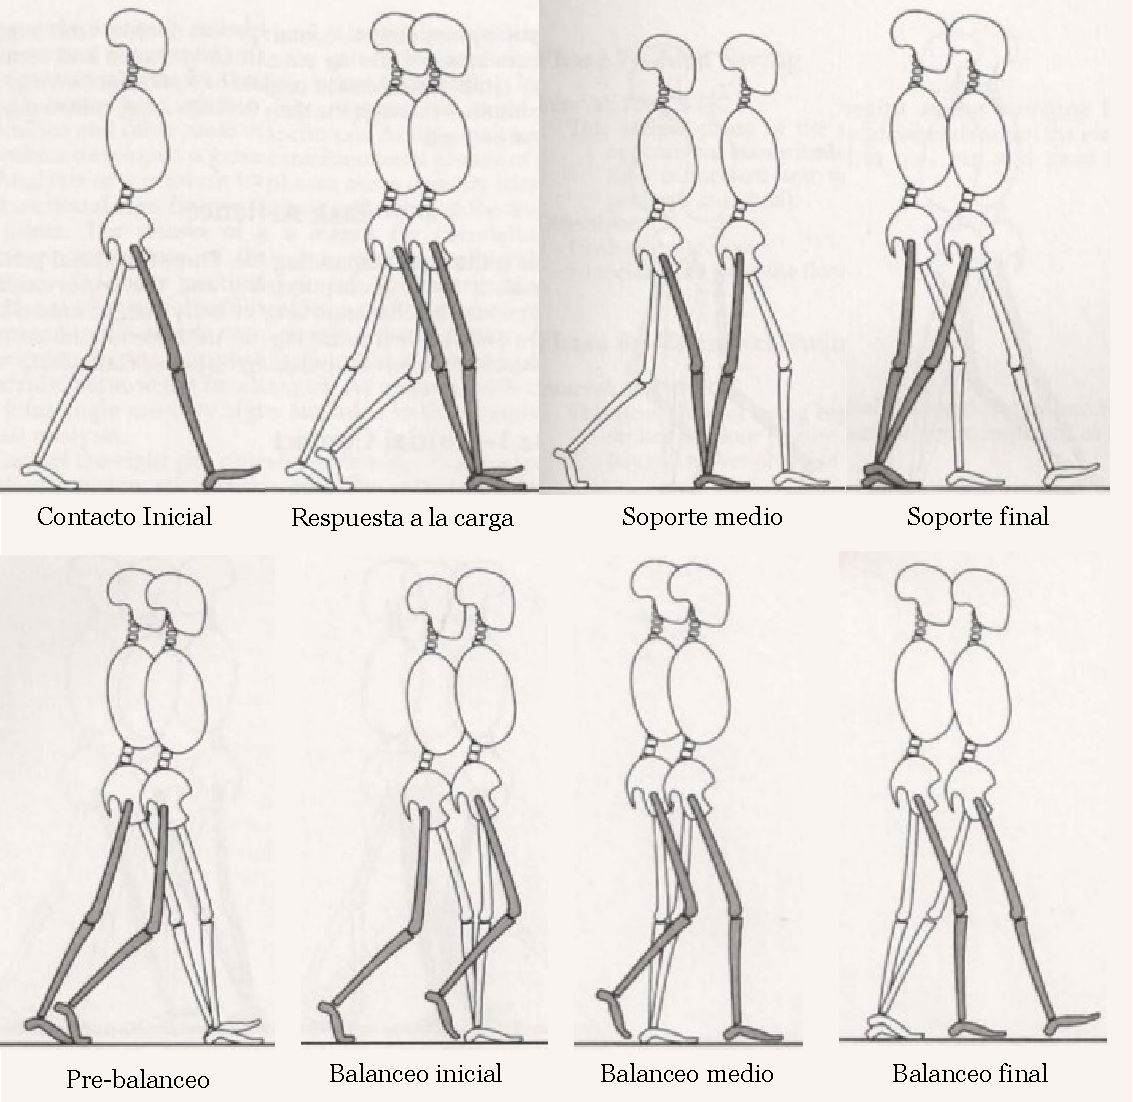
\includegraphics[width = \textwidth]{imagenes/ciclo_marcha}
    \caption{Ilustración del ciclo de la marcha, tomado de \citep{perry}}
    \label{fig:ciclo_marcha}
\end{figure}



\begin{figure}
    \centering
    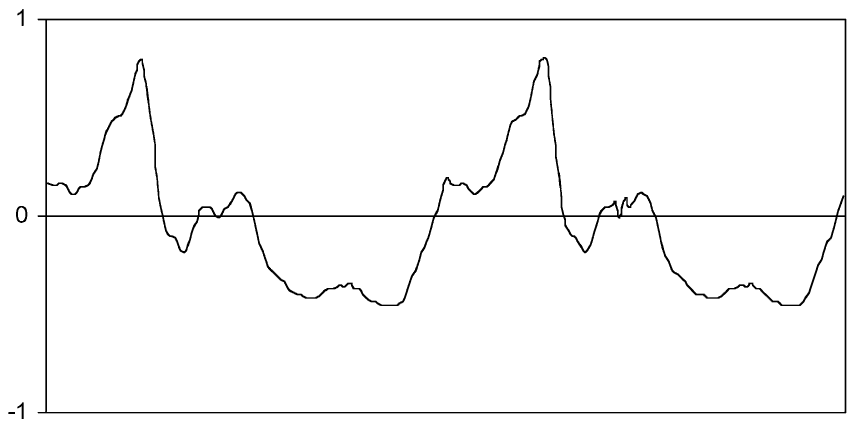
\includegraphics[width = 0.75\textwidth]{imagenes/menz_acceleration}
    \caption{Aceleración vertical de la cadera, tomado de \citep{menz}}
    \label{fig:menz_acc_ver}
\end{figure}

A grandes rasgos, el pico de mayor tamaño representan el momento donde se transfiere el peso de una pierna a la otra, existe en esa fase un tiempo muy corto donde el cuerpo está casi en caída libre (la gravedad es la principal fuerza de locomoción). Esto es seguido del contacto inicial y la aceptación de la carga. La valle largo y llano corresponde al fase de balanceo, donde una pierna se adelanta hacia la posición de contacto inicial.

Al utilizar sensores para recolectar datos de la marcha, se puede aplicar gran cantidad de herramientas matemáticas para caracterizar el movimiento e intentar encontrar \emph{patrones} útiles al diagnosticar condiciones clínicas. 

Otra estrategia al estudiar la marcha no solo consiste en obtener una descripción del ciclo, sino intentar modelar el mecanismo que la genera. \cite{dejnabadi} considera la marcha como un proceso automático, controlado por el \emph{sistema nervioso central}, el cual reduce la complejidad de planar el movimiento al artificalmente disminuir los grados de libertad del cuerpo. En el modelo propuesto, se regenerar un patron el moviento al seleccionar los parámetros cadencia y logitud del paso, todas las velocidades se pueden obtener como una combinación de estos parámetros. La ventaja de contar con un modelo de la causa del patrón de la marcha es poder caracterizar y estudiar la desviaciones de este modelo para identificar afectaciones. 



\section[Herramienta de diagnóstico]{Análisis de la marcha como herramienta de diagnóstico}

Tal como se menciona en la sección anterior, la marcha produce una serie de patrones, tanto en las variables cinemáticas como dinámicas. El análisis de dichos patrones puede utilizarse como herramienta de diagnostico. Tome por ejemplo un daño en los músculos pretibiales, principales encargados de elevar el piel al final de la fase de balanceo (figura \ref{fig:heel_rocker}). Sin la acción de este músculo la punta del pie, y no el talón, es el primero en hacer contacto con el piso, esto impide una transferencia de carga efectiva y aumenta el esfuerzo de la marcha.

Para compensar la función de los músculos pretibiales, el patrón de la marcha se ve modificado, un ejemplo es la marcha del personaje \emph{el vagabundo} de Charles Chaplin \footnote{En \url{https://www.youtube.com/watch?v=L277pNm3Y4w} se puede encontrar un extracto de Charles Chaplin interpretando al \emph{vagabundo}}. En este caso los cuadriceps hacen un esfuerzo extra para aumentar el ángulo de la rodilla, generando un pequeño latigazo, que permite un contacto inicial con la planta del pie (horizontal), evitando así arrastrar la punta del pie.

El patrón de la marcha de el personaje \emph{el vagabundo} parece ser una combinación de varias afectaciones, sin embargo su análisis permitiría encontrarlas y aplicar tratamientos correctivos: ejercicios, calzado ortopédico, operaciones. 

\begin{figure}
    \centering
    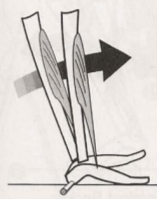
\includegraphics[width=0.2\textheight]{imagenes/heel_rocker}
    \caption{Función de los músculos pretibiales. Tomado de \citep{perry}}
    \label{fig:heel_rocker}
\end{figure}

Los siguientes son casos concretos encontrados en la literatura, donde se utiliza el estudio de la marcha junto con análisis por computadora para detectar afectaciones especificas.

\subsection{Enfermedades neurodegenerativas}

\cite{arif} plantea la hipótesis de que la edad afecta la estabilidad de marcha y propone analizar la entropía de la señal de aceleración, generada por un sensor colocado en la zona lumbar, para cuantificar la estabilidad de la marcha. Los resultados siguieren que la entropía de la marcha aumenta según la edad. Pero en general la entropía aumenta según la velocidad de la marcha, para compensar este hecho, las personas intentan optimizar la estabilidad al disminuir velocidad de la marcha. En general las personas mayores desarrollan una cadencia\footnote{Cadencia: cantidad de pasos por unidad de tiempo} menor que las personas jóvenes. 

Ahora bien, la edad no es el único factor que podría afectar la estabilidad de la marcha y su cadencia. Personas que sufren de enfermedades degenerativas, como esclerosis, Alzheimer, traumatismos cerebrales, entre otros, sufren de marcha inestable, por ejemplo \cite{ren} y \cite{wu} analizan la fluctuaciones el el ritmo de la marcha, con lo cual logra identificar, a través del estudio de la marcha, a personas con padecimientos neurodegenerativos y de esta forma proponer acciones para mejorar su calidad de vida. \cite{yang} realiza un aporte semejante, pero estudiando la rotación axial y estabilidad de la marcha al dar la vuela.  

\subsection{Daños en ligamentos}

\cite{christian} muestra como el patrón característico de la marcha se ve afectado por daños en ligamentos de las extremidades inferiores, específicamente se estudió el ligamento cruzado anterior de la rodilla. Una reducción con PCA \footnote{\emph{Principal Component Analysis}} y una máquina de soporte vectorial permitió identificar aquellas personas con una lesión en dicho ligamento. 

El análisis de marcha también puede ayudar a mejorar el rendimiento deportivo. Tal como señala \cite{perry}, los atletas empujan el funcionamiento normal del cuerpo hasta sus límites, esto se evidencia en el patrón de la marcha, generando mayores fuerzas en las articulaciones y arcos de movimiento más amplios. Entender cómo la práctica deportiva afecta los patrones de movimiento podría ayudar a disminuir el riesgo de lesiones y mejorar el desempeño.  

\subsection{Atrofia por hemofilia}

\cite{forneris} presenta un estudio pionero en el campo, donde analiza los patrones de la marcha de pacientes de hemofilia entre los 4 y 18 años. Sus resultados logran caracterizar el progreso causado por la enfermedad y esta información podría utilizarse para diagnosticar de manera temprana daños en articulaciones y atrofia por hemofilia, además de permitir desarrollar terapias personalizadas. 

\subsection{Parálisis cerebral}

Los pacientes de parálisis cerebral suelen sufrir dificultades en la locomoción, el análisis de marcha permite identificar estas dificultades y permite planear tratamientos efectivos para evitar la atrofia y mejorar la calidad de vida del paciente. \cite{sangeux} lista las desviaciones más comunes encontradas en el patrón de la marcha para articulaciones específicas, lo cual permite encontrar el origen de dicha desviación y personalizar la terapia.


\section[Métodos de recolección]{Métodos de recolección de datos}

Los métodos de recolección de datos se puede clasificar según su portabilidad en portables y no-portables (\emph{wearable} y \emph{non-wearable}) y según su tecnología en procesamiento de imagen, sensores de fuerza, sensores de inercia y electromiogramas. \citep{muro}

Los sistemas de captura de movimiento no portables tienen la ventaja de ser muy precisos y permiten medir directamente las variables buscadas. Al estar instalados en ambientes controlados, como laboratorios o salas de mediciones clínicas y conducidas por profesionales, las mediciones realizadas son menos propensas a sufrir ruido, perturbaciones y son repetibles. También, al estar conectados a la red eléctrica, el consumo de potencia no es una limitación. Como desventaja, al ser un ambiente controlado y generalmente pequeño, el patrón natural de la marcha se puede ver afectado y el equipo es muy costoso. \citep{muro}

Los sistemas de captura de movimiento portables tiene la ventaja de permitir recolectar datos durante las actividades diarias normales del paciente, son mucho más baratos que los sistemas no portables y no necesitan de personal para controlar el uso del dispositivo. Como desventaja, el consumo de potencia es una preocupación importante, pues deben funcionar de manera independiente a la red. Son muy suceptibles al ruido y las interferencias externas y al medir las variables deseadas de manera indirecta, se necesitan algoritmos complejos para recuperar los datos deseados. \citep{muro}

\subsection{Procesamiento de imagen}

Está conformado por una o varias cámaras, estas pueden ser cámaras digitales comunes RGB, basadas en el tiempo de eco para generar un mapa de profundidad (como kinect de Microsoft) o utilizar escáner láser. Algunos sistemas pueden necesitar marcadores y estos pueden ser activos o pasivos, ejemplos son \cite{prakash, yang2}. \citep{muro}

Debido al bajo costo de las cámaras digitales y software robusto para el análisis de imágenes, esta tecnología es muy utilizada. Como ejemplo se puede mencionar a \cite{hoang}, donde dos cámaras se colocan antiparalelas viendo una superficie de caminado y \cite{li} y \cite{mrozowski} donde se colocan las cámaras de manera perpendicular. 

Como ejemplo de sistemas ópticos con marcadores, la figura \ref{fig:pris_mocap} muestra el sistema de captura óptica de movimiento  del Pris-Lab, Escuela de Ingeniería Eléctrica, Universidad de Costa Rica. Consiste en cámaras infrarrojas y un traje con marcadores pasivos muy reflectivos en el rango de frecuencia de las cámaras. 

%\begin{figure}
%    \centering
%    \includegraphics[width = 0.6\textwidth]{images/pris_mocap}
%    \caption{Sistema MoCap del Pris-Lab, UCR}
%    \label{fig:pris_mocap}
%\end{figure}

\subsection{Sensores de presión y fuerza}

Comúnmente consiste en alfombras de sensores o plantillas que se ajustan al calzado. Permiten medir el vector de fuerza transmitido al piso \footnote{Según la Tercera Ley de Newton} producido al caminar sobre la superficie. Además de permitir cálculos sobre las variables espacio temporales de la marcha y segmentar el ciclo de marcha, permiten, utilizando cinemática inversa y en combinación con algún otro sistema de captura de movimiento, calcular las fuerzas y torques en articulaciones, por ejemplo \cite{mizoguchi}.

\subsection{Sensores de inercia}

Consisten de acelerómetros y giroscopios (IMU) colocados en diversos puntos del cuerpo del paciente, conectados a un microcontrolador. Ejemplos se encuentran en \cite{menz}, \cite{arif}, \cite{senanayake}, \cite{latt}, \cite{mazza}, \cite{hu}, entro otros. Son muy sencillos y por eso resulta práctico utilizarlos, sin embargo solo pueden reportar unas pocas variables cinemáticas y se pierde toda información sobre la posición del paciente.

\cite{yuan} presenta un método con el cual se puede conocer la posición del usuario y muchas de las variables cinemáticas, para esto utiliza 8 IMUs colocados sobre el cuerpo.

\subsection{Electromiografía}

La electromiografía es la recolección de los pequeños impulsos eléctrico generados por los músculos al contraerse. Se utilizan electrodos no invasivos colocados sobre la piel para poder recolectar estas señales. Se suelen utilizar en combinación con algún otro método de captura del movimiento, para asociar el patrón de la marcha con la activación del los músculos. \cite{muro}

\subsection{Otros medios de recolección}

\cite{krigslund} desarrolló un método para conocer la orientación de segmentos rígidos utilizado un dispositivo RFID con antenas bipolares. Al ser pasivos, estos dispositivos podrían utilizarse por largo tiempo, sin embargo se necesita equipo alrededor para recolectar los datos. 

También se utilizan galgas de compresión, sensores piezoeléctricos y sensores capacitivos, para intentar estimar la posición de las articulaciones. \citep{muro}


\section[Software disponible]{Software disponible para estudios sobre la marcha}

En muchos casos, los estudios sobre la marcha se realizan con software específico para el experimento, desarrollado en alguna plataforma como Matlab (este es el caso de la mayoría de trabajos analizados) \citep{cuaya, mrozowski, eskinazi, senanayake, prakash, punt, menguc, bruijn}. Por ejemplo \cite{menz} utiliza SPSS, un software de análisis estadístico predictivo. \cite{mizoguchi}, por ejemplo, utiliza nMotion Musculous de NAC Image Technology, con lo cual calcula la fuerza de activación de cada músculo y después hace un análisis estadístico, no especifica en cual plataforma, pero podría ser incluso en una hoja de cálculo. 

En un ambiente clínico, existen programas especializados en ayudar al practicante en el diagnóstico y seguimiento de las dificultades motoras. Por ejemplo se tiene 3D Gait, EliteClinic Systems, TEMPLO Contemplas, Medical Motion Pro-Trainer Motion analysis, Motion Monitor Gait Analysis, entre otros. Desde la ingeniería, han existido propuestas de software para facilitar el estudio clínico, por ejemplo \cite{hayla} y \cite{senanayake}, sin embargo no parecen tener mucho éxito, principalmente debido a la dificultada de validar dicho software e incluir una cantidad suficiente de \emph{feautures} para hacerlo atractivo en el ámbito clínico. Desde la estrategia de generar un modelo sobre la marcha para utilizarlo como referencia, \cite{vieira} entrena una red neuronal para facilitar el análisis clínico de la marcha.

Alrededor del estudio de la marcha, existen pequeños paquetes de software con funciones muy específicas, por ejemplo \cite{eskinazi} presenta SCMT, un paquete para simular la interacción musculo esquelética en las articulaciones, utilizando datos reales.

Hasta el momento, no se ha encontrado un software libre que permita realizar estudios de la marcha de manera integra, es decir, desde la recolección de los datos hasta su análisis y presentación de resultados. 


